The crab drive layer consists of the hardware components that include a main drive motor that is responsible for steering the wheel motors that move the wheels. The drive system interface is responsible for communicating with the camera interface in the imaging subsystem, supplying directions to the main motor, and providing the cart with holonomic capabilities.

\begin{figure}[h!]
	\centering
 	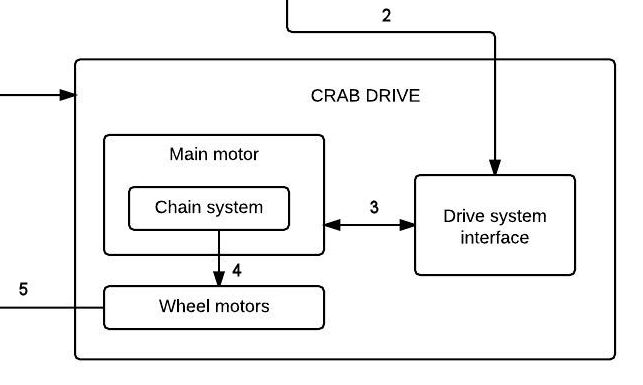
\includegraphics[width=0.60\textwidth]{images/crab}
 \caption{Crab drive layer}
\end{figure}

\subsection{Drive System Interface Subsystem}
The drive system interface is designed to communicate with the navigation subsystem's camera interface. it will get  navigation data from the camera interface to steer the main drive motor as well as receiving feedback information for the wheel orientations.

\begin{figure}[h!]
	\centering
 	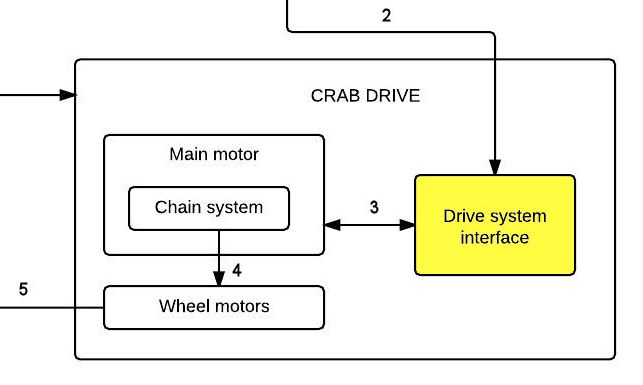
\includegraphics[width=0.60\textwidth]{images/crab_interface}
 \caption{Drive system interface subsystem}
\end{figure}

\subsubsection{Assumptions}
Assumptions made are as follows:
\begin{itemize}
	\item The drive system interface will receive accurate navigation data from the camera interface.
	\item The drive system interface will receive accurate feedback data from the main motor about wheel orientation.
\end{itemize}

\subsubsection{Responsibilities}
The drive system interface subsystem's responbilities are as follows:
\begin{itemize}
	\item Send navigation data to the main motor.
	\item Receive wheel feedback data.
\end{itemize}

\subsubsection{Subsystem Interfaces}

\begin {table}[H]
\caption {Drive system interface subsystem interfaces} 
\begin{center}
    \begin{tabular}{ | p{1cm} | p{6cm} | p{3cm} | p{3cm} |}
    \hline
    ID & Description & Inputs & Outputs \\ \hline
    \#2 & Receive navigation data  & \pbox{3cm}{Camera interface} & \pbox{3cm}{Main motor}  \\ \hline
    \#3 & Receive wheel data & \pbox{3cm}{Main motor} & \pbox{3cm}{Camera interface}  \\ \hline
    \end{tabular}
\end{center}
\end{table}
\newline


\subsection{Main Motor Subsystem}
The main motor will contain a chain system that is responsible for steering the cart and maintaining a consistent orientation for all of the wheels.

\begin{figure}[h!]
	\centering
 	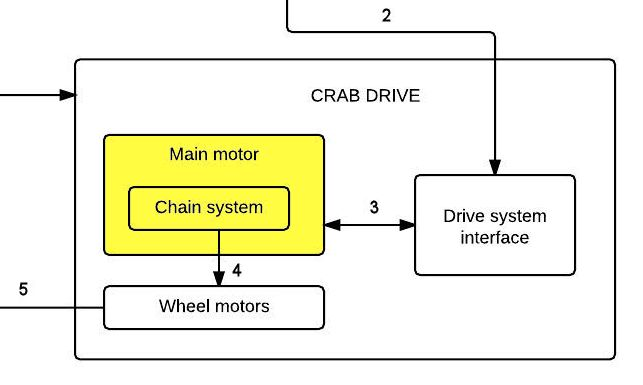
\includegraphics[width=0.60\textwidth]{images/crab_motor}
 \caption{Main motor subsystem}
\end{figure}

\subsubsection{Assumptions}
Assumptions made are as follows:
\begin{itemize}
	\item The main motor will correctly steer the wheels with the chain/belt system.
	\item The main motor will have a method to accurately keep wheel orientation data.
\end{itemize}

\subsubsection{Responsibilities}
The main motor subsystem's responbilities are as follows:
\begin{itemize}
	\item Receive steering instructions from the drive system interface and accurately perform instructions.
\end{itemize}

\subsubsection{Subsystem Interfaces}

\begin {table}[H]
\caption {Main motor subsystem interfaces} 
\begin{center}
    \begin{tabular}{ | p{1cm} | p{6cm} | p{3cm} | p{3cm} |}
    \hline
    ID & Description & Inputs & Outputs \\ \hline
    \#4 & Steer wheels  & \pbox{3cm}{Drive system interface} & \pbox{3cm}{Wheel motors}  \\ \hline
    \#3 & Feedback data  & \pbox{3cm}{N/A} & \pbox{3cm}{Drive system interface}  \\ \hline
    \end{tabular}
\end{center}
\end{table}
\newline


\subsection{Wheel Motors Subsystem}
The wheel motors is designed to drive the wheels at an appropriate speedt to follow the user using information sent by the main motor.

\begin{figure}[h!]
	\centering
 	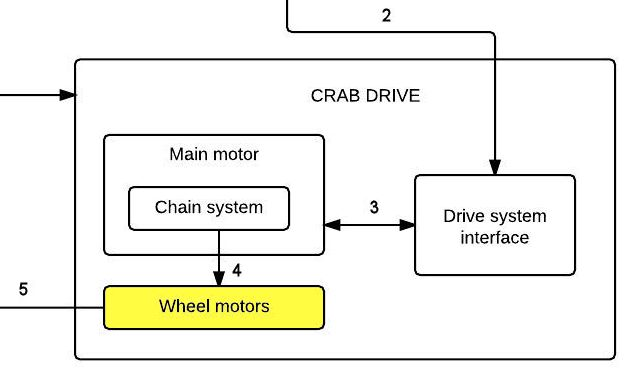
\includegraphics[width=0.60\textwidth]{images/crab_wheel}
 \caption{Wheel motors subsystem}
\end{figure}

\subsubsection{Assumptions}
Assumptions made are as follows:
\begin{itemize}
	\item The wheel motors will be able to decide how fast to spin to achieve an appropriate speed.
	\item The wheel motors will only spin in one direction as the chain/belt system will control steering.
\end{itemize}

\subsubsection{Responsibilities}
The wheel motors subsystem's responbilities are as follows:
\begin{itemize}
	\item Drive the wheels to follow a user at an appropriate speed.
\end{itemize}

\subsubsection{Subsystem Interfaces}

\begin {table}[H]
\caption {Wheel motors subsystem interfaces} 
\begin{center}
    \begin{tabular}{ | p{1cm} | p{6cm} | p{3cm} | p{3cm} |}
    \hline
    ID & Description & Inputs & Outputs \\ \hline
    \#5 & Receive drive data  & \pbox{3cm}{Chain system} & \pbox{3cm}{Wheels}  \\ \hline
    \end{tabular}
\end{center}
\end{table}